\section{Interactive Video Stream Context Management and QA Types}\label{sec:stream_context}

\begin{figure}[t]
    \centering
    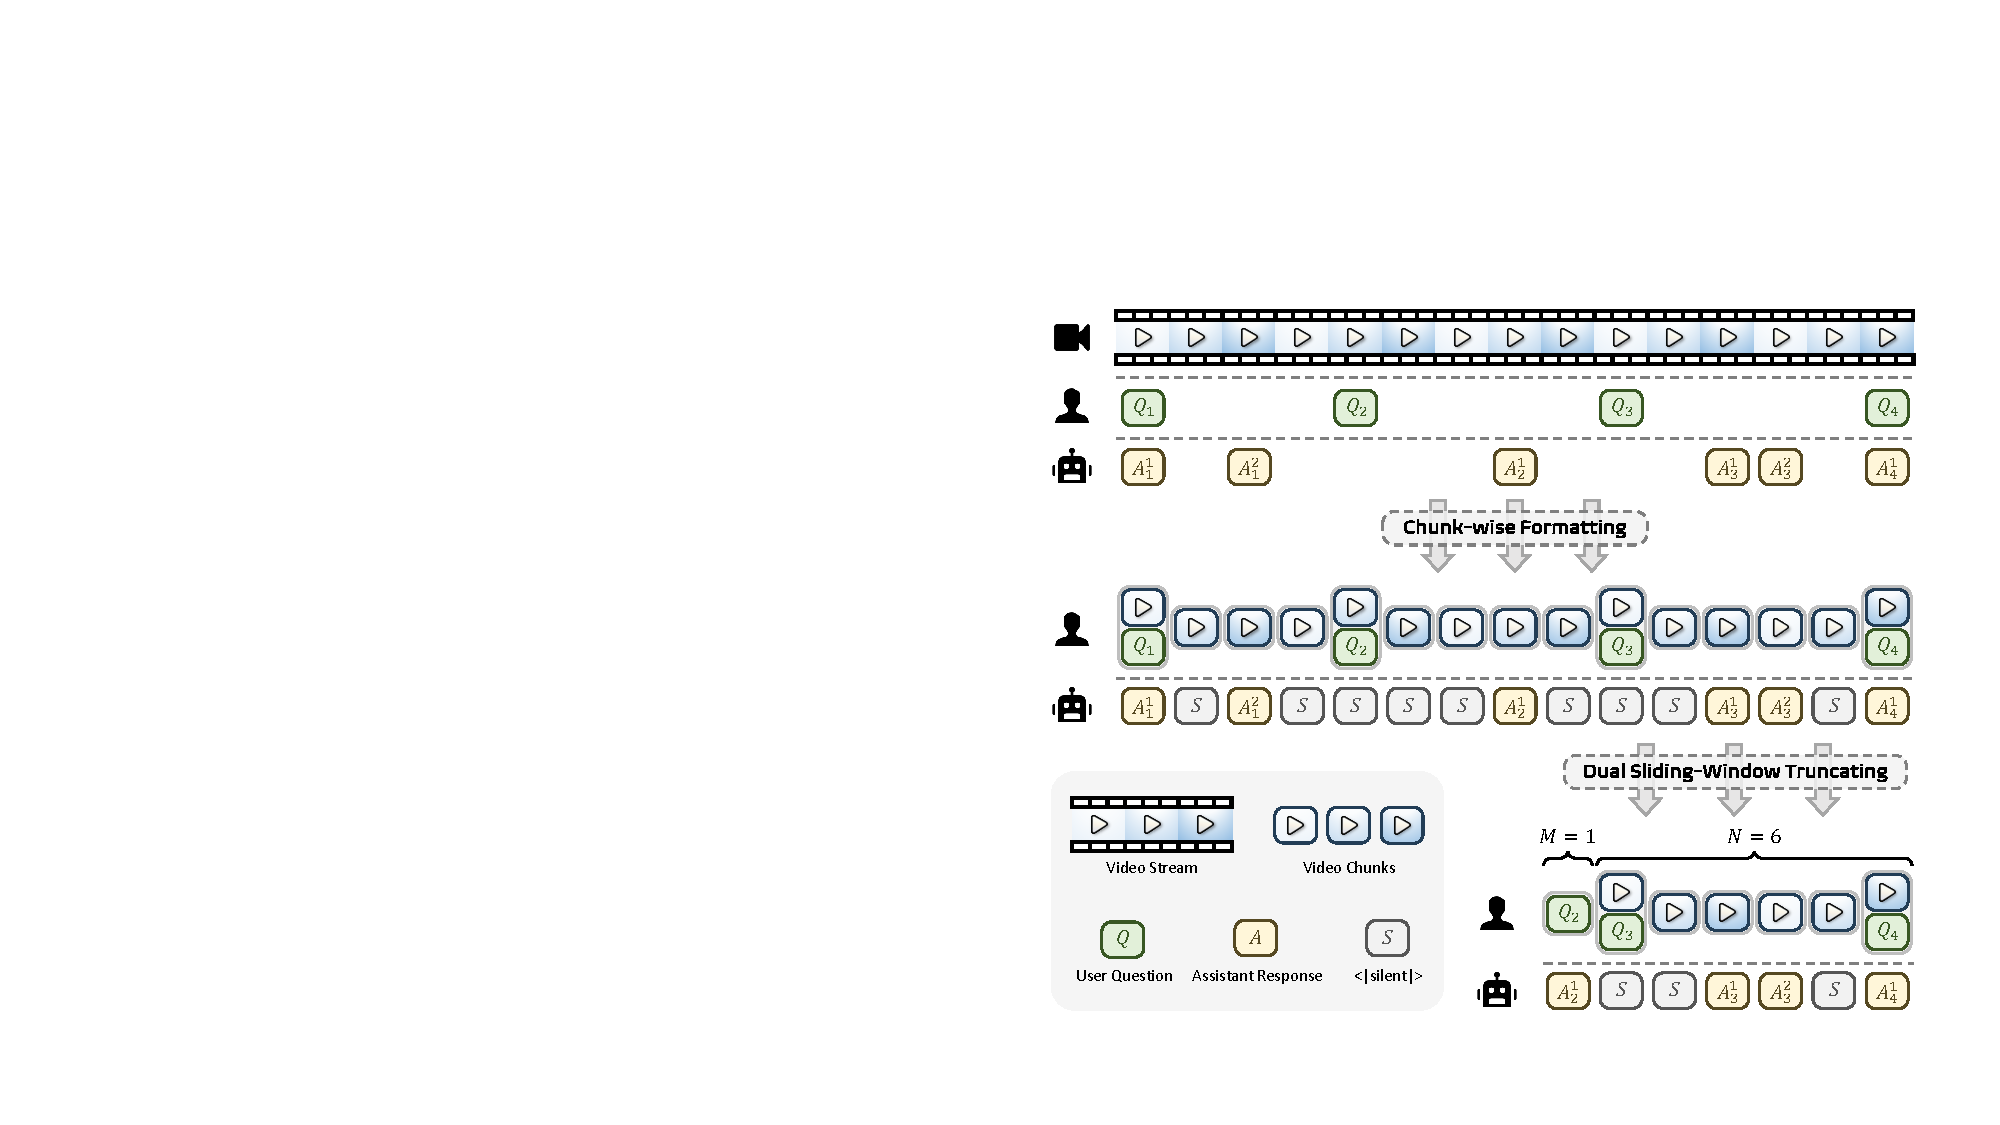
\includegraphics[width=\textwidth]{img/3_context_management_2.pdf}
    \caption{Overview of our Interactive Video Stream Context Management mechanism. The framework uses a dual sliding-window strategy, where $N$ denotes the length of the video window, and $M$ denotes the number of recent QA groups retained in the interaction history outside the video window.}
    \label{fig:Interactive_Video_Stream_Context_Management}
\end{figure}

Building continuous and timely visual interaction modeling for streaming scenarios is highly challenging. In streaming video understanding, both the input video and the interaction history between the user and the model (\ie, the assistant) grow continuously over time, making the continuity unbounded. However, the context window of an LLM is fundamentally limited, and an excessively long context can slow inference, thereby compromising timeliness. To address this trade-off, AURA introduces an Interactive Video Stream Context Management mechanism, as illustrated in Figure~\ref{fig:Interactive_Video_Stream_Context_Management}. Based on this mechanism, three streaming QA modes are defined.

\subsection{Interactive Video Stream Context Management}\label{subsec:interactive_video_stream_context_management}

\paragraph{Chunk-wise Conversational Format.}
Because the video stream is collected in small temporal chunks (\eg, one chunk per second), we organize the context in a chunk-wise conversational format. For each video chunk, if a user question is issued at that time, the question and the corresponding video chunk are packaged together into a user message. Otherwise, the user message contains only the video chunk and no text. Each user message is followed by an assistant message. If there is an assistant response at that time step, the assistant message contains the response text; otherwise, it is filled with a special token, \texttt{<|silent|>}, indicating that the model remains silent at that moment.

\paragraph{Dual Sliding-Window Strategy.}
To manage the unbounded growth of the streaming video and interaction history, we adopt a dual sliding-window strategy over both the video stream and the QA interaction stream. For the video stream, we maintain a sliding window that keeps only the most recent $N$ seconds of video. Because visual tokens are highly dense and user-relevant information is typically associated with recent visual content, $N$ is set to a relatively small value (\eg, $N=30$). In contrast, QA interactions are text-based, token-efficient, and often carry critical user intent and historical context. Therefore, outside the video window, we maintain a separate sliding window over QA interactions that preserves the most recent $M$ QA groups (\eg, $M=10$), where a QA group is defined as a user question together with all subsequent non-silent assistant responses. If the total video duration does not exceed $N$ seconds, the full history is retained. Otherwise, the context is truncated jointly by the video and QA windows. For the $M$ QA groups that fall outside the $N$-second video window, all video chunks and \texttt{<|silent|>} tokens are discarded, and only the valid textual content of the user and assistant messages is preserved. Overall, this dual sliding-window strategy preserves important historical information while controlling the total context length and enabling efficient computation.

\begin{figure}[t]
    \centering
    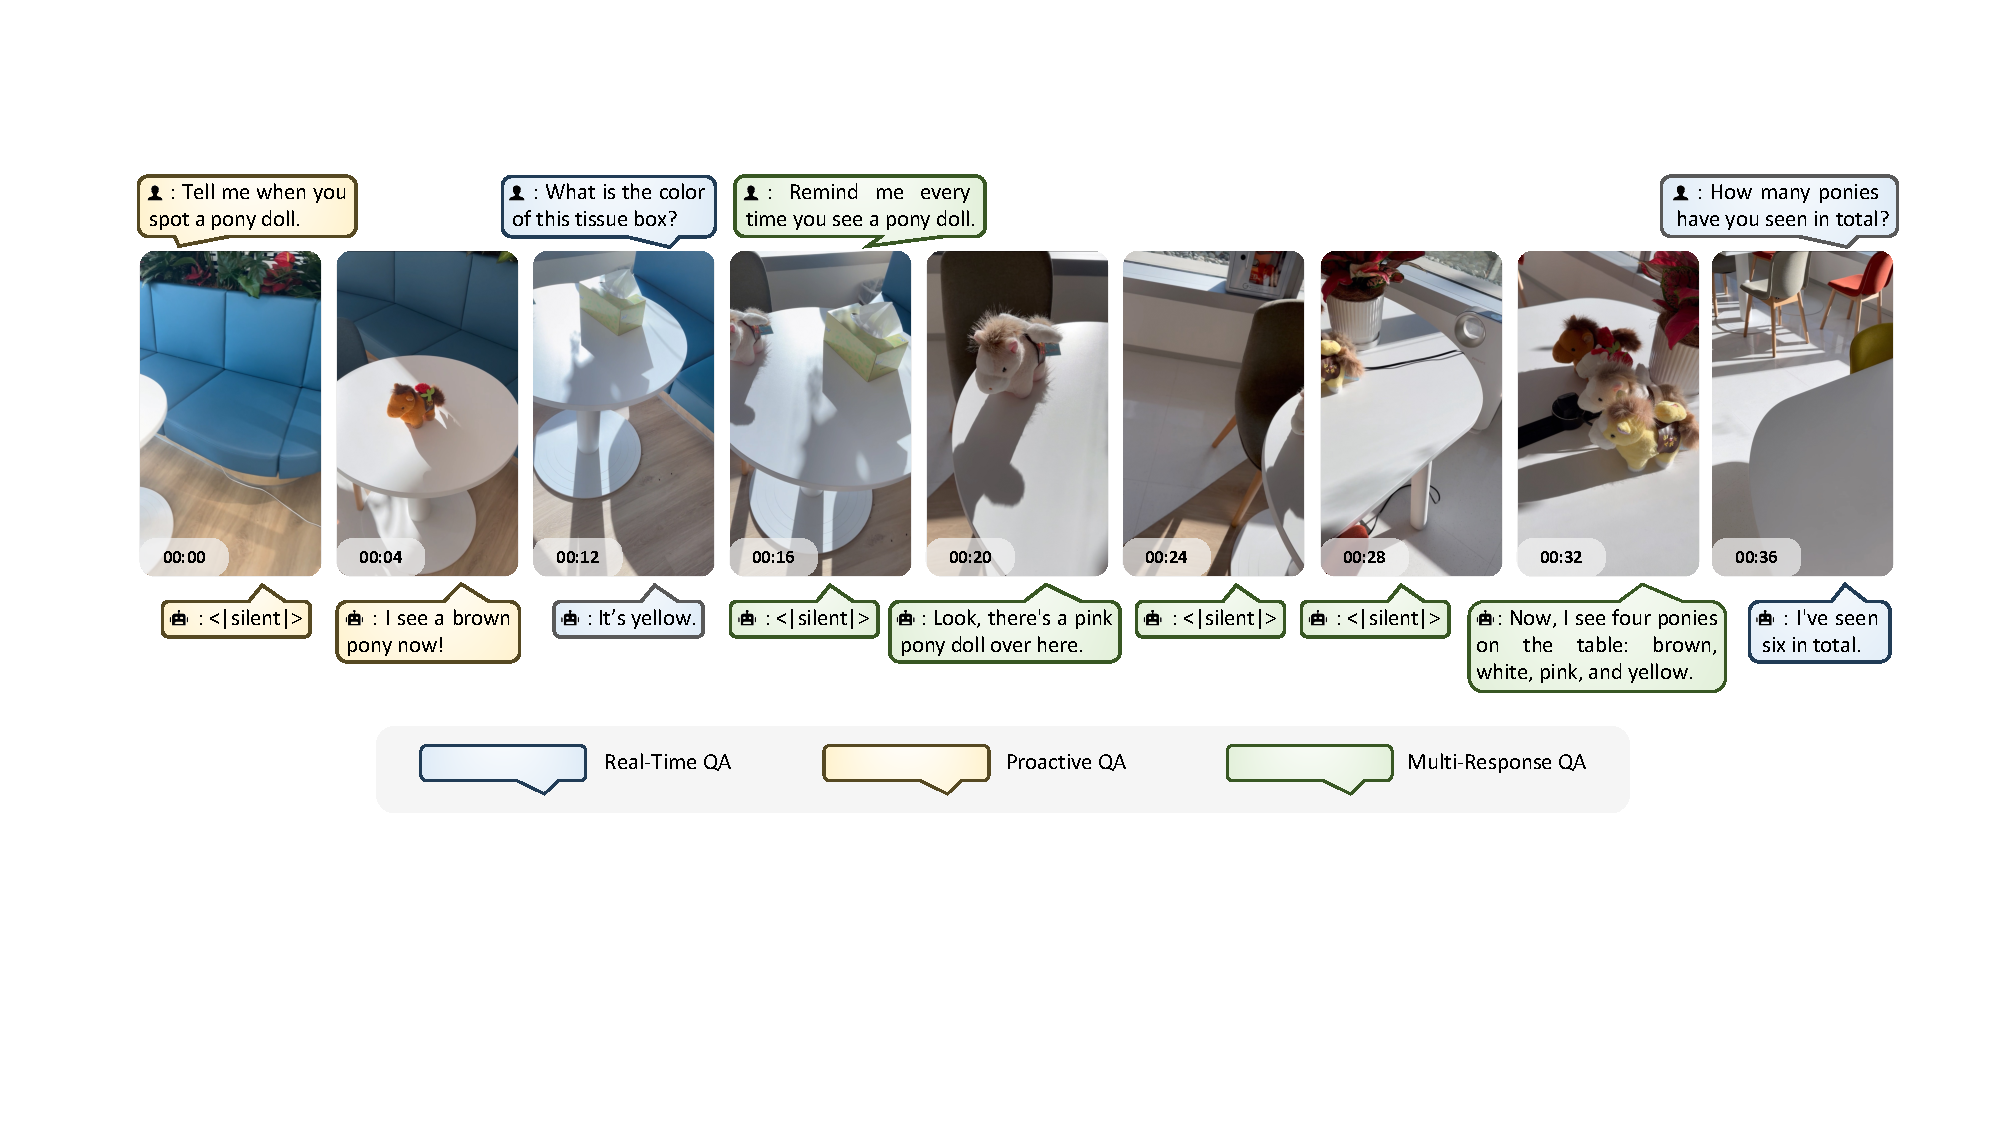
\includegraphics[width=\textwidth]{img/3_qa_examples_2.pdf}
    \caption{The figure illustrates three types of streaming QA interactions. 
\textbf{Real-Time QA} produces a single immediate response at the query time. 
\textbf{Proactive QA} produces a single delayed response after sufficient future evidence is observed. 
\textbf{Multi-Response QA} continuously tracks evolving events and produces multiple responses over time without requiring repeated queries.}
    \label{fig:QA_examples}
\end{figure}


\subsection{Streaming QA Types}





Based on the context management mechanism in Section~\ref{subsec:interactive_video_stream_context_management}, user-assistant interaction is no longer restricted to the traditional turn-taking paradigm, where a single response is generated immediately after each query. Instead, both the user and the assistant can interact asynchronously over a continuous video stream, resembling natural human conversation.
In such streaming settings, user queries exhibit diverse temporal dependencies on visual information. Some queries can be resolved immediately based on the current or previous observations, while others require waiting until sufficient evidence emerges in the future. Additionally, certain queries pertain to ongoing events, requiring the model to continuously monitor the scene and produce multiple responses as new information becomes available, without repeated user input.

These interaction patterns reflect diverse response requirements in streaming settings, varying in both response timing and frequency. Accordingly, we categorize streaming QA interactions into three types according to the timing and multiplicity of responses for each query:

\textbf{(1) Real-Time QA}, where the model produces a single immediate response grounded in the currently available or previously observed visual context;

\textbf{(2) Proactive QA}, where the model remains silent after receiving the query and generates a single response only after sufficient visual evidence has been accumulated;

\textbf{(3) Multi-Response QA}, where the model generates multiple responses over time as new visual information becomes available.

Examples of these interaction types are illustrated in Figure~\ref{fig:QA_examples}. Together, these three categories form the foundation of our data construction pipeline (Section~\ref{sec:data_pipe}), enabling the model to learn diverse response behaviors under streaming conditions.








